We emulate the climatological mean response, because that is the response of interest in assessments of climate change impacts. Because the year-over-year response can be significantly different from the forced climatological one, we do not use information from year-to-year variability but instead emulate the aggregated mean yield in each 30-year simulation. Changes in these time-averaged yields are also considerably smoother than those in year-to-year yield response, making emulation relatively straightforward. 

In the GGCMI Phase II simulation output dataset, year-over-year responses to weather are indeed quantitatively distinct from responses to climatological shifts. 
The differences are especially significant for temperature: yield response to short-term temperature fluctuations are often significantly stronger than those to climatological shifts.
This behavior is illustrated in Figure \ref{fig:yearvclim}, which shows irrigated (left) and rainfed (right) maize in a representative location in Iowa, with black lines and open circles showing the climatological mean responses and colored lines and solid circles those for the 30 individual years in selected scenarios. Yields are three times as sensitive to year-over-year temperature fluctuations as they are to climatological  temperature shifts (1.9 vs.\ 0.6 tons ha$^{-1}$/K in the baseline climate, Figure \ref{fig:yearvclim}, left), with both responses rising slightly at warmer temperatures.
Yield sensitivity to precipitation, on the other hand, is similar at both timescales (Figure \ref{fig:yearvclim}, right), but also highly nonlinear, with losses becoming more severe with increasing dryness
%The differences are especially significant for temperature, with yield fluctuations generally stronger in response to short-term temperature fluctuations than in response to changes in climatological means. 
%Yield sensitivity to precipitation, on the other hand, is similar for both year-over-year and climatological changes (Figure \ref{fig:yearvclim}, right), though both are highly nonlinear and losses become more severe with increasing dryness. 

While differences in year-over-year and climatological temperature responses can arise for many reasons, including memory in the crop model and lurking covariates, the most reasonable explanation is that the regressor here, mean growing-season temperature, does not fully describe the conditions that affect crop yields. That is, changes in growing-season temperature \textit{means} in the forced and unforced cases may involve different changes in growing-season temperature \textit{distributions} \citep[e.g.][]{Ruane2016}. 
The similarity of responses to precipitation perturbations across timescales is then expected, because changes in precipitation distributions affect yields less than do those in temperature. 
Crops respond not to precipitation but to soil moisture, which integrates on timescales of weeks or even months \textcolor{red}{cite ?}. 
Previous studies have suggested that in all but very arid regions, yields are not sensitive to how precipitation is distributed within a month \citep{Glotter14}.

In the GGCMI Phase II experiment, the imposed perturbations involve no changes in underlying distributions (reasonable since summertime change are expected to be small \textcolor{red}{cite ?}), but year-over-year variations are \textcolor{red}{XX}. 
Note that year-over-year spreads in yields do become wider in highly impacted climate states in GGCMI Phase II (Figure 2), but only because yield responses to both temperature and precipitation perturbations are nonlinear. 
Higher sensitivity in conditions of extreme climate stress results in greater year-to-year variance in yields.


%Note however that for both precipitation and temperature, year-over-year reponses are stronger in conditions of larger climate impacts (higher T or lower W), so that variance in  

%Note that the GGCMI Phase II training dataset does not capture potential changes in climate variability, because all simulations are run with fixed offsets from the historical climatology.
%However, prior work has suggested that mean changes are the dominant drivers of climatological crop yield shifts in all but arid regions \citep[e.g.][]{Glotter14}.
%Critically for emulation, the mean-climatological yield can easily be related to the mean-climatological shift in temperature or precipitation in the GGCMI Phase II dataset.

%For example, the stronger year-over-year response to temperature under warmer conditions also manifests as a wider distribution of yearly yields (Figure \ref{fig:yearly}) within a 30-year simulation even though the variance in input temperates is unchanged. 
%Likewise for precipitation changes, strong decreases in precipitation results in a widening of the distribution in yields even though the variance in precipitation is decreasing (from approximately 60 cm yr-1 to 30 cm yr-1 in this example). 
%In both cases show in the Figure (Figure \ref{fig:yearly}), the year-over-year response is nonlinear, getting stronger with more severe mean climate shifts. 
%The strengthening of crop sensitivity under severe climate shifts causes distribution of modeled crop yields becomes wider, even when underlying climate variability is fixed.
%For temperature, that strengthening year-over-year response adds a complication to emulating when using a non-stationary climate scenario where mean climate gradually warms.
%In contrast for precipitation, the year over year response is locally similar to the climatological response.  
%Note that since we emulate mean climatological-yields, we do not capture any of these higher-order moment changes in yield in this study.

%While differences in year-over-year and climatological temperature responses can arise for many reasons, including memory in the crop model and lurking covariates, the most reasonable explanation is that the regressor here, mean growing-season temperature, does not fully describe the conditions that affect crop yields. That is, changes in growing-season temperature \textit{means} may involve different changes in growing-season temperature \textit{distributions} in the forced and unforced cases \citep[e.g.][]{Ruane2016}. 
%are associated with different changes in temprein the chara that short-term temperature fluctuations are associated with different associated distributions of daily growing-season daily weather . 
%In the GGCMI Phase II experiment, the imposed perturbations involve no changes in underlying distributions (reasonable since summertime change are expected to be small \cite{XX}), but year-over-year variations are \textit{XX}. Note that year-over-year distributions of yields do become wider in highly impacted climate states in GGCMI Phase II (Figure \ref{fig:yearly}), but only because yield responses to both temperature and precipitation perturbations are nonlinear.
%It is expected that precipitation perturbations would produce more similar responses on year-over-year and climatological scales, because changes in precipitation distributions affect yields less than do those in temperature. Crops respond not to precipitation but to soil moisture, which integrates on timescales of weeks or even months \textcolor{red}{cite \cite{XX}}. 
%Previous studies have suggested that in all but very arid regions, yields are not sensitive to how precipitation is distributed within a month \citep{Glotter14}.

%The first critical design choice for our emulators is concerned with temporal aggregation.
%We construct our emulator of 30-year climatological mean yields because most economic models project impacts at some aggregate temporal scale (decades or larger) or utilize some temporally aggregated climate projection as their input.
%The GGCMI Phase II model experiment parameter sweep was designed to provide a training dataset for emulation that is structured in a way conducive to this temporal aggregation.

%you're saying that the year-over-year would add noise but not change your fit. But, I think this is why you talk about the nonlinearity of the year-over-year response, because in some cases it WOULD add bias. right? If the year-over-year response is the same as the mean response it's fine. If it's different from the mean response and not changing, I think even that adds bias, because your "noise" is then not stationary - its relationship to the mean response differs depending on temperature. If it's different from the mean response and changing, then it's definitely not stationary.


%%%%%%%%%%%%%%%%%%%%%%%%%%%%%%%%%%%%%%%%%%%%%%%%%%%%%%%%%%%%%%%
%%%%%%%%%%%%%%%%%%%%%%%%%%%%%%%%%%%%%%%%%%%%%%%%%%%%%%%%%%%%%%%
%%%%%%%%%%%%%%%%%%%%%%%%%%%%%%%%%%%%%%%%%%%%%%%%%%%%%%%%%%%%%%%
%%%%%%%%%%%%%%%%%%%%%%%%%%%%%%%%%%%%%%%%%%%%%%%%%%%%%%%%%%%%%%%
%  OLD UNUSED 
%%%%%%%%%%%%%%%%%%%%%%%%%%%%%%%%%%%%%%%%%%%%%%%%%%%%%%%%%%%%%%%
%%%%%%%%%%%%%%%%%%%%%%%%%%%%%%%%%%%%%%%%%%%%%%%%%%%%%%%%%%%%%%%
%%%%%%%%%%%%%%%%%%%%%%%%%%%%%%%%%%%%%%%%%%%%%%%%%%%%%%%%%%%%%%%
%%%%%%%%%%%%%%%%%%%%%%%%%%%%%%%%%%%%%%%%%%%%%%%%%%%%%%%%%%%%%%%



%The same general principal applies to a lesser degree the precipitation dimension however in this case it is more manifestly an artifact of sampling range in the historical period (Figure \ref{fig:yearvclim}, right).
%Furthermore, the year-over-year response is nonlinear with baseline climate: while the climatological response is nearly the same in T+0 to T+6 scenarios, evolving only from XX-XX tons ha$^{-1}$/K, the year-over-year response rises by over a quarter, from 1.9 to 2.5 tons ha$^{-1}$/K.
%The first critical design choice for our emulators is concerned with temporal aggregation.
%We construct our emulator of 30-year climatological mean yields because most economic models project impacts at some aggregate temporal scale (decades or larger) or utilize some temporally aggregated climate projection as their input.
%The GGCMI Phase II model experiment parameter sweep was designed to provide a training dataset for emulation that is structured in a way conducive to this temporal aggregation.
%you're saying that the year-over-year would add noise but not change your fit. But, I think this is why you talk about the nonlinearity of the year-over-year response, because in some cases it WOULD add bias. right? If the year-over-year response is the same as the mean response it's fine. If it's different from the mean response and not changing, I think even that adds bias, because your "noise" is then not stationary - its relationship to the mean response differs depending on temperature. If it's different from the mean response and changing, then it's definitely not stationary.
%We emulate the yield response to C, T, W, and N at the 30-year climatological mean level.
%, 2) the year-over-year response is not the same as the climatological response (Figure 2), 3) if we included the year-over-year response it's both noisier, making emulation harder, and can also actually bias the emulated response
%then you close by saying the GGCMI dataset lets you use a relatively simple form that converges well. That transitions you to the emulation section
%Three important distinctions are made between the year-to-year yield response and the climatological-mean yield response.
%Note however that for both precipitation and temperature, year-over-year reponses are stronger in conditions of larger climate impacts (higher T or lower W), so that variance in  
%Note that the GGCMI Phase II training dataset does not capture potential changes in climate variability, because all simulations are run with fixed offsets from the historical climatology.
%However, prior work has suggested that mean changes are the dominant drivers of climatological crop yield shifts in all but arid regions \citep[e.g.][]{Glotter14}.
%Critically for emulation, the mean-climatological yield can easily be related to the mean-climatological shift in temperature or precipitation in the GGCMI Phase II dataset.
%For example, the stronger year-over-year response to temperature under warmer conditions also manifests as a wider distribution of yearly yields (Figure \ref{fig:yearly}) within a 30-year simulation even though the variance in input temperates is unchanged. 
%Likewise for precipitation changes, strong decreases in precipitation results in a widening of the distribution in yields even though the variance in precipitation is decreasing (from approximately 60 cm yr-1 to 30 cm yr-1 in this example). 
%In both cases show in the Figure (Figure \ref{fig:yearly}), the year-over-year response is nonlinear, getting stronger with more severe mean climate shifts. 
%The strengthening of crop sensitivity under severe climate shifts causes distribution of modeled crop yields becomes wider, even when underlying climate variability is fixed.
%For temperature, that strengthening year-over-year response adds a complication to emulating when using a non-stationary climate scenario where mean climate gradually warms.
%In contrast for precipitation, the year over year response is locally similar to the climatological response.  
%Note that since we emulate mean climatological-yields, we do not capture any of these higher-order moment changes in yield in this study.


%Some models share a common genealogy, but have since branched and developed independently, and will be treated independently in this work. 
%Minor differences in historical rainfall across the different reanalysis products used result in differences in the precipitation shift in the parameter-sweep. 
%Atmospheric CO$_2$ and applied nitrogen fertilizer take uniform, static values globally for each 30-year simulation case.
%Sampling across the parameter sweep is heterogeneous across models so the resultant training dataset size differs across models. 
%(See Table \ref{table:models} for number of 30-year simulations).


\begin{figure*}[ht]
\centering
    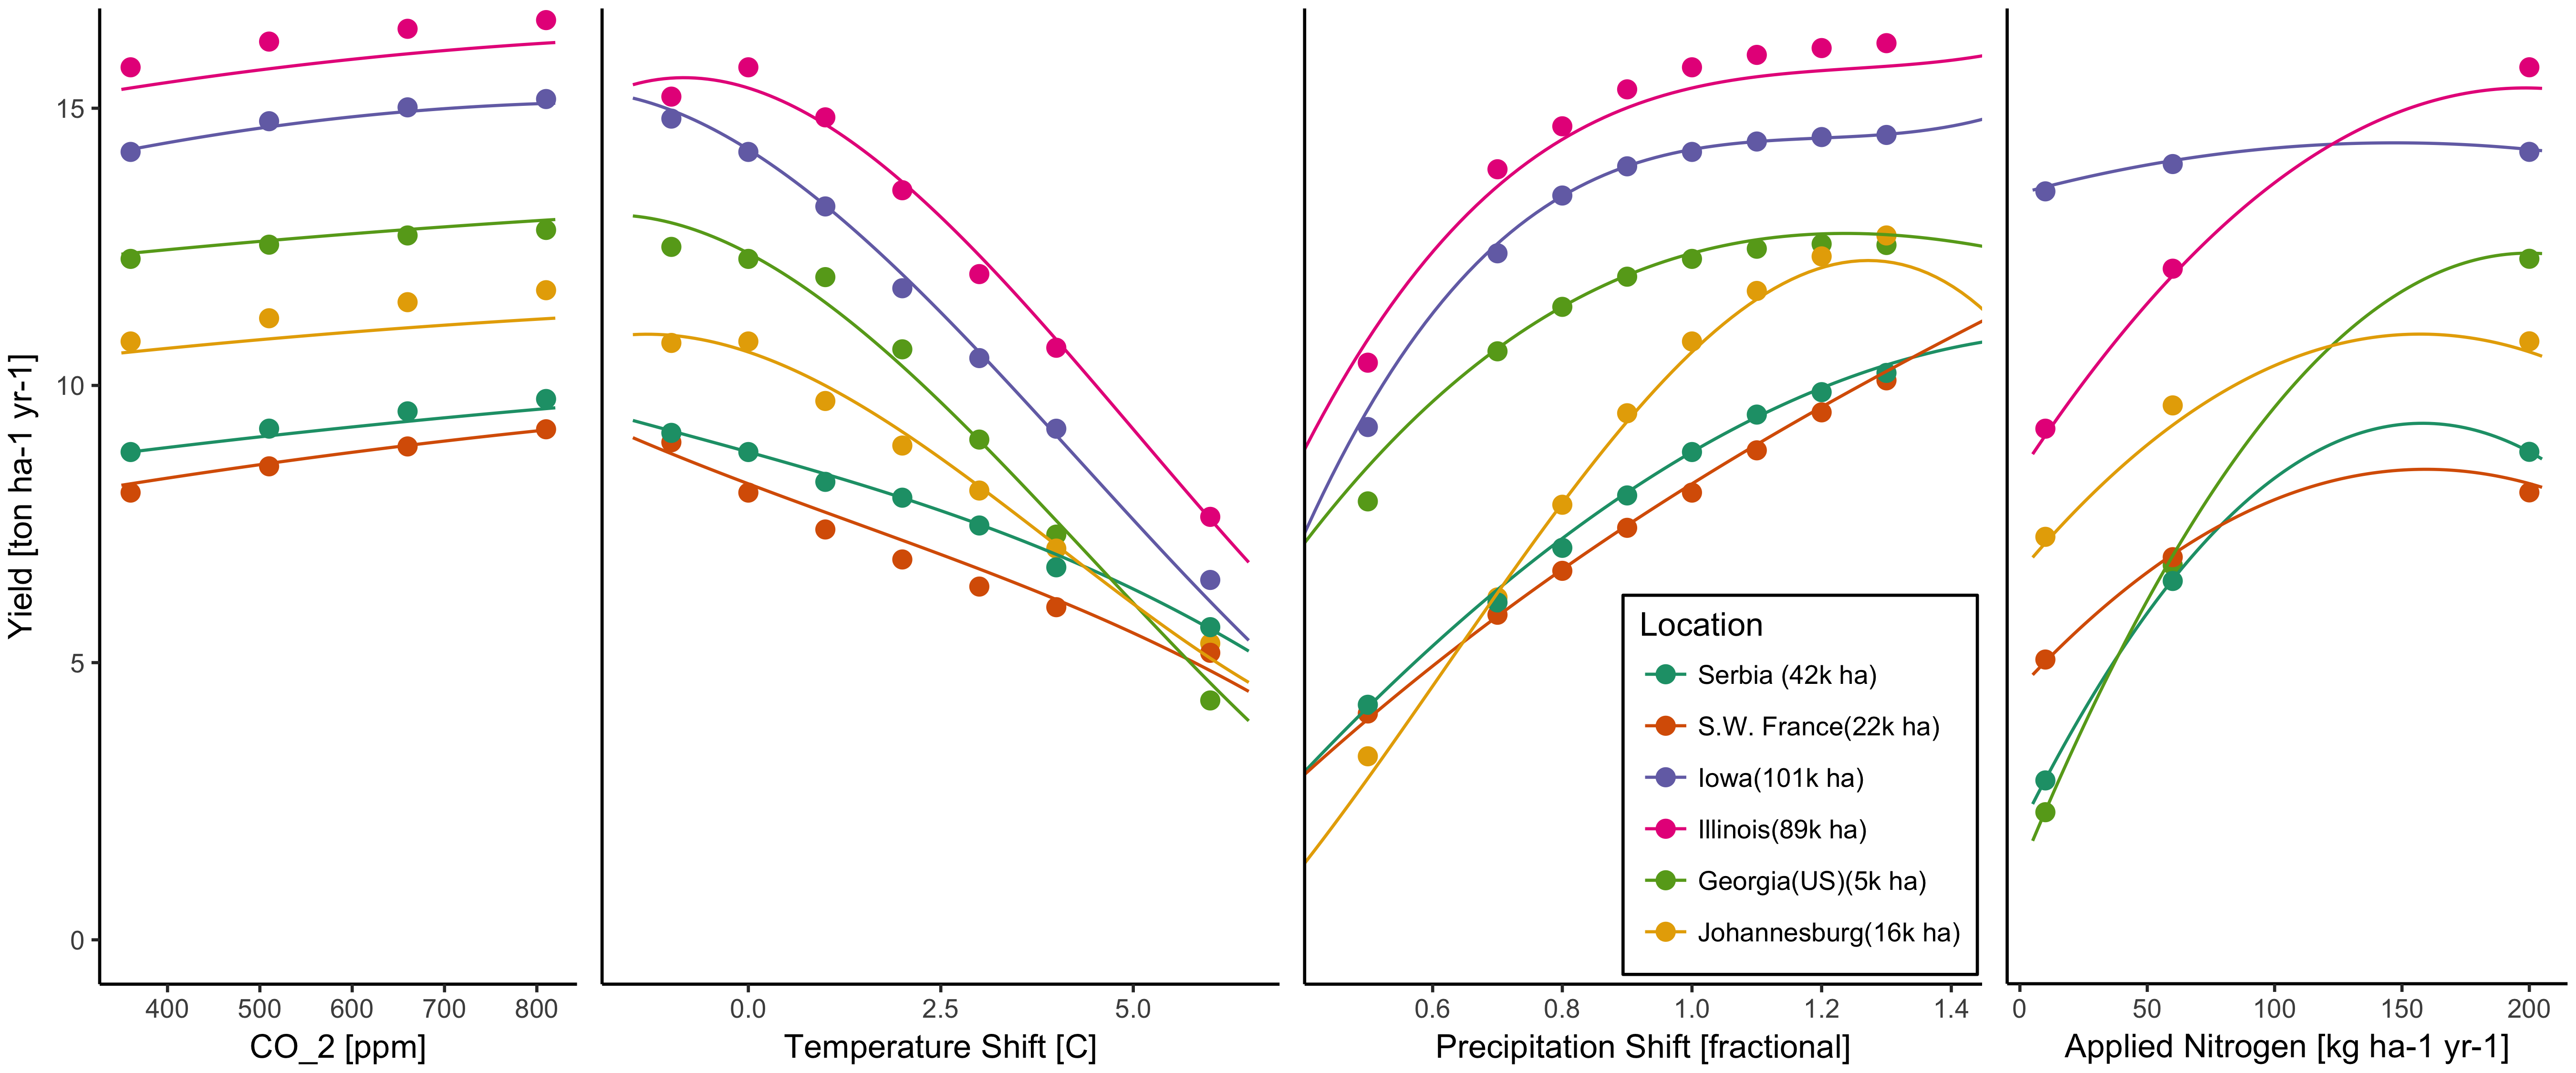
\includegraphics[width=16cm]{figures/regression_areas.png}
    \caption{Illustration of spatial variations in yield response successfully captured by the emulator. 
    We show rainfed maize in the pDSSAT model in six example locations selected to represent high-cultivation areas around the globe. 
    Legend includes hectares cultivated in each selected grid cell. 
    Each panel shows variation along a single variable, with others held at baseline values. 
    Dots show climatological mean yields and lines the results of the full 4D emulator of Equation \ref{eqn:features_original}. 
    In general the climatological response surface is sufficiently smooth that it can be represented within the sampled variable space by the simple polynomial used in this work. 
    Extrapolation can however produce misleading results. 
    Nitrogen fits in some cases may not be realistic at intermediate values given limited sampling. 
    For more detailed emulator assessment, see Appendix B.}
   \label{fig:regression}
\end{figure*}

\begin{figure*}[ht]
\centering
    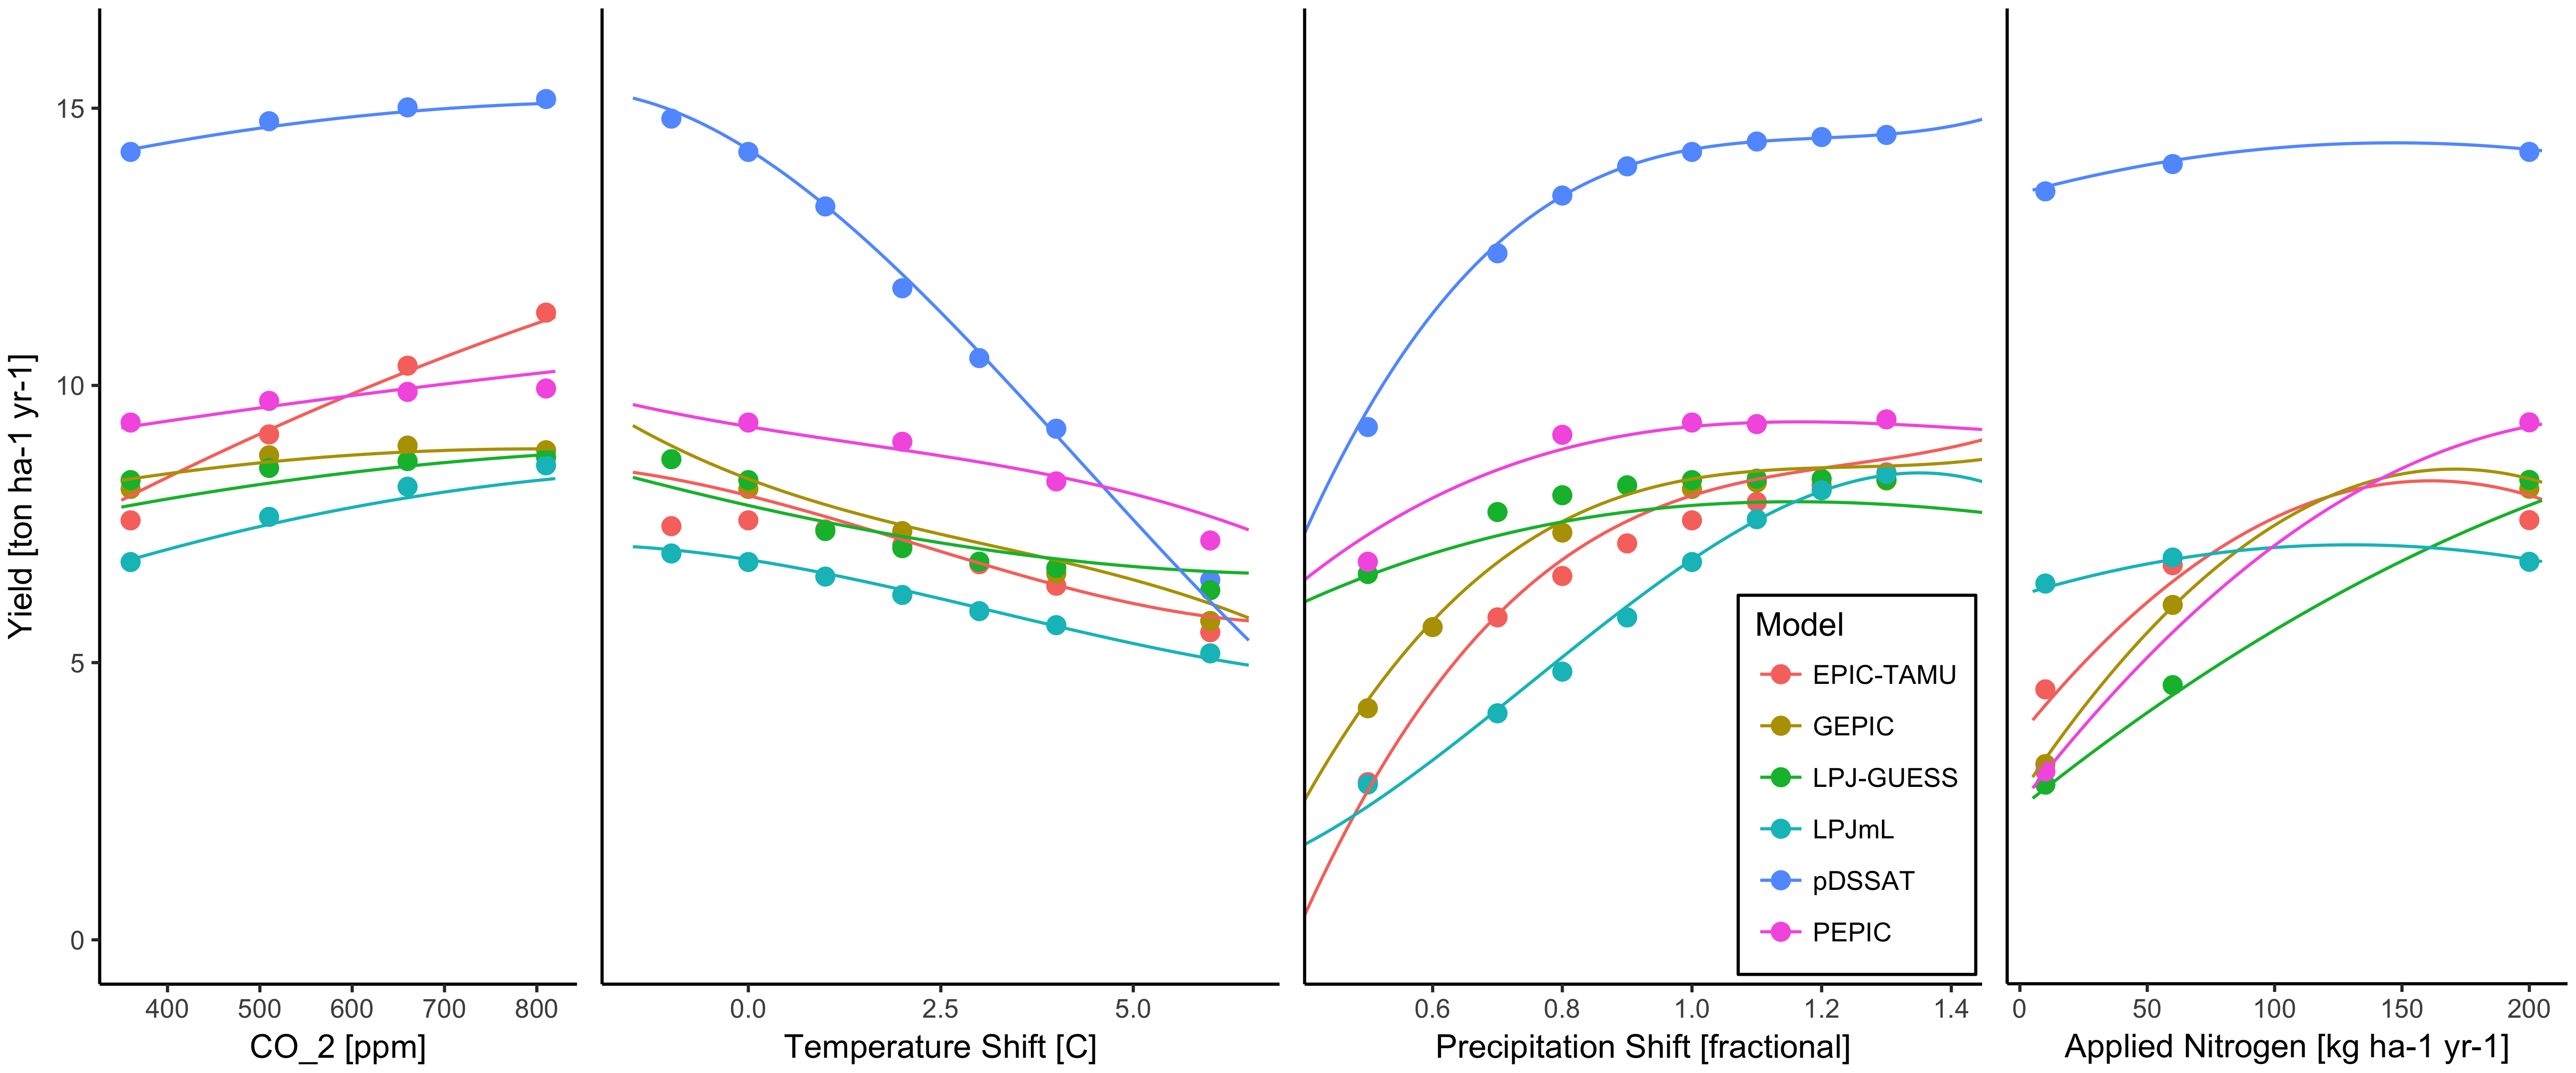
\includegraphics[width=16cm]{figures/regression_model.png}
    \caption{Illustration of across-model variations in yield response successfully captured by the emulator. 
    Figures shows simulations and emulations from six models for rainfed maize in the same Iowa grid cell shown in Figure \ref{fig:regression}, with the same plot conventions. 
    Models that do not simulate the nitrogen dimension are omitted for clarity. 
    Note that models are uncalibrated, increasing spread in absolute yields. 
    While most model responses can readily emulated with a simple polynomial, some response surfaces diverge slightly from the polynomial approach (e.g.\ LPJ-GUESS here) and lead to emulation error, though error generally remains small relative to inter-model uncertainty. 
    For more detailed emulator assessment, see Appendix B. 
    As in Figure \ref{fig:regression}, extrapolation out of the sample space is potentially problematic.}
   \label{fig:regression_iowa}
\end{figure*}

\begin{figure}[ht]
\centering
   \caption{Example showing distinction between crop yield responses to year-to-year and climatological mean precipitation shifts. 
   Figure shows rainfed maize for a representative high-yield region (nine adjacent grid cells in northern Iowa) from the pDSSAT model, for the baseline 1981-2010 historical climate (gray) and for the scenario of maximum and minimum precipitation change (brown and green). 
   Other covariates are held at baseline values.
   Open black circles mark climatological mean yield values for all seven precipitation scenarios (W -50\%, -30\%, -20\%, -10\%, W, +10\%, +20\%, +30\%). 
   Colored lines show total least squares linear regressions of year-over-year variations in each scenario. 
   Bold Black line shows the emulator fit through the climatological mean values.}
   \label{fig:yearvclimpr}
\end{figure}

    {Totals} & {9} & {8} & {8} & {8} & {9} & {8} & {5240 | 3378}\\


We include interaction terms (both linear and higher-order) because past studies have shown them to be significant effects. 
To limit over-fitting and unstable parameter estimation, we apply a feature selection procedure (described below) that reduces the potential 34-term polynomial (for the rainfed case) to 23 terms.
We regress 30-year climatological mean yields against a third-order polynomial in C, T, W, and N with interaction terms. 


\begin{align}
    \label{eqn:features_original}
    Y\ = \ & K_{1}  \\
    + \ & K_{2} C      + K_{3} T      + K_{4} W      + K_{5} N   \nonumber \\
    + \ & K_{6} C^2    + K_{7} T^2    + K_{8} W^2    + K_{9} N^2 \nonumber \\
    + \ & K_{10} C W   + K_{11} C N   + K_{12} T W   + K_{13} T N   + K_{14} W N \nonumber \\
    + \ & K_{15} C T   + K_{16} T^3   + K_{17} W^3   + K_{18} C^3   + K_{19} N^3 \nonumber \\
    + \ & K_{20} T W N + K_{21} T^2 W + K_{22} W^2 T + K_{23} W^2 N + K_{24} C W N \nonumber \\
    + \ & K_{25} C T N + K_{26} N^2 C + K_{27} N^2 T + K_{28} N^2 W + K_{29} T^2 N \nonumber \\
    + \ & K_{30} T^2 C + K_{31} W^2 C + K_{32} C^2 W + K_{33} C^2 T + K_{34} C^2 N \nonumber
\end{align}


%The resulting statistical model (Equation \ref{eqn:features_final}) is used for all grid cells, models, and rainfed crops. 
%(The regressions for irrigated crops do not contain the W terms and the models that do not sample the nitrogen levels omit the N terms.)

%\begin{align}
%    \label{eqn:features_final}
%    Y\ = \ & K_{1}  \\
%       + \ & K_{2}  C     + K_{3}  T     + K_{4}  W     + K_{5}  N   \nonumber \\
%       + \ & K_{6}  C^2   + K_{7}  T^2   + K_{8}  W^2   + K_{9}  N^2 \nonumber \\
%       + \ & K_{10} C W   + K_{11} C N   + K_{12} T W   + K_{13} T N + K_{14} W N \nonumber \\ % lost 1 term, CT
%%      + \ & K_{15} T^3   + K_{16} W^3   + K_{17} T W N  \nonumber \\ % lost 2 terms, C^3 and N^3
%       + \ & K_{18} T^2 W + K_{19} W^2 T + K_{20} W^2 N  \nonumber \\ % lost 2 terms, CWN and CTN
%%      + \ & K_{21} N^2 C + K_{22} N^2 T + K_{23} N^2 W  \nonumber    % lose 6 terms: T^2N and T^2C, W^2C, 3 C^2 terms
%\end{align}


\label{table:ASE}
\begin{tabular}{l | cc | cc | cc | cc | cc} 
\hline
{} & \multicolumn{2}{c|}{\textbf{Maize}} & \multicolumn{2}{c|}{\textbf{Soy}}& \multicolumn{2}{c |}{\textbf{Rice}} & \multicolumn{2}{c |}{\textbf{S. Wheat}} & \multicolumn{2}{c}{\textbf{W. Wheat}} \\
\textbf{Model}     & WM (\%)& MD (\%)& WM (\%)& MD (\%)& WM (\%)& MD (\%)& WM (\%)& MD (\%)& WM (\%) & MD (\%) \\ \hline
\textbf{CARAIB}    & 0.00  & 1.71  & 0.02  & 2.39  & 0.03  & 2.95  & 0.02  & 4.40  & 0.01  & 2.36  \\ \hline
\textbf{EPIC-TAMU} & 0.00  & 4.30  & 0.01  & 6.24  & 0.00  & 3.35  & 0.01* & 6.82* & 0.01  & 3.51  \\ \hline
\textbf{JULES}     & 0.11  & 6.13  & 0.01  & 10.2  & 0.01  & 6.97  & 0.04  & 15.1  & NA    & NA    \\ \hline
\textbf{GEPIC}     & 0.00  & 5.78  & 0.00  & 3.75  & 0.01  & 5.64  & 0.01  & 6.76  & 0.01  & 7.01  \\ \hline
\textbf{LPJ-GUESS} & 0.00  & 1.78  & NA    & NA    & NA    & NA    & 0.05  & 6.22  & 0.02  & 3.35  \\ \hline
\textbf{LPJmL}     & 0.00  & 9.44  & 0.00  & 3.25  & 0.01  & 8.37  & 0.01  & 9.83  & 0.01  & 4.98  \\ \hline
\textbf{pDSSAT}    & 0.00  & 2.93  & 0.05  & 3.02  & 0.01  & 3.97  & 0.01  & 2.97  & 0.01  & 4.67  \\ \hline
\textbf{PROMET}    & 0.01  & 4.19  & 0.00  & 6.03  & 0.01  & 9.85  & 0.01  & 7.04  & 0.01  & 3.68   \\ \hline
\textbf{PEPIC}     & 0.00* & 3.71* & 0.00* & 2.80* & 0.00* & 2.89* & 0.00* & 4.83* & 0.02* & 6.70*  \\ \hline
\end{tabular}
\end{table*}



\begin{figure}[ht]
\centering
   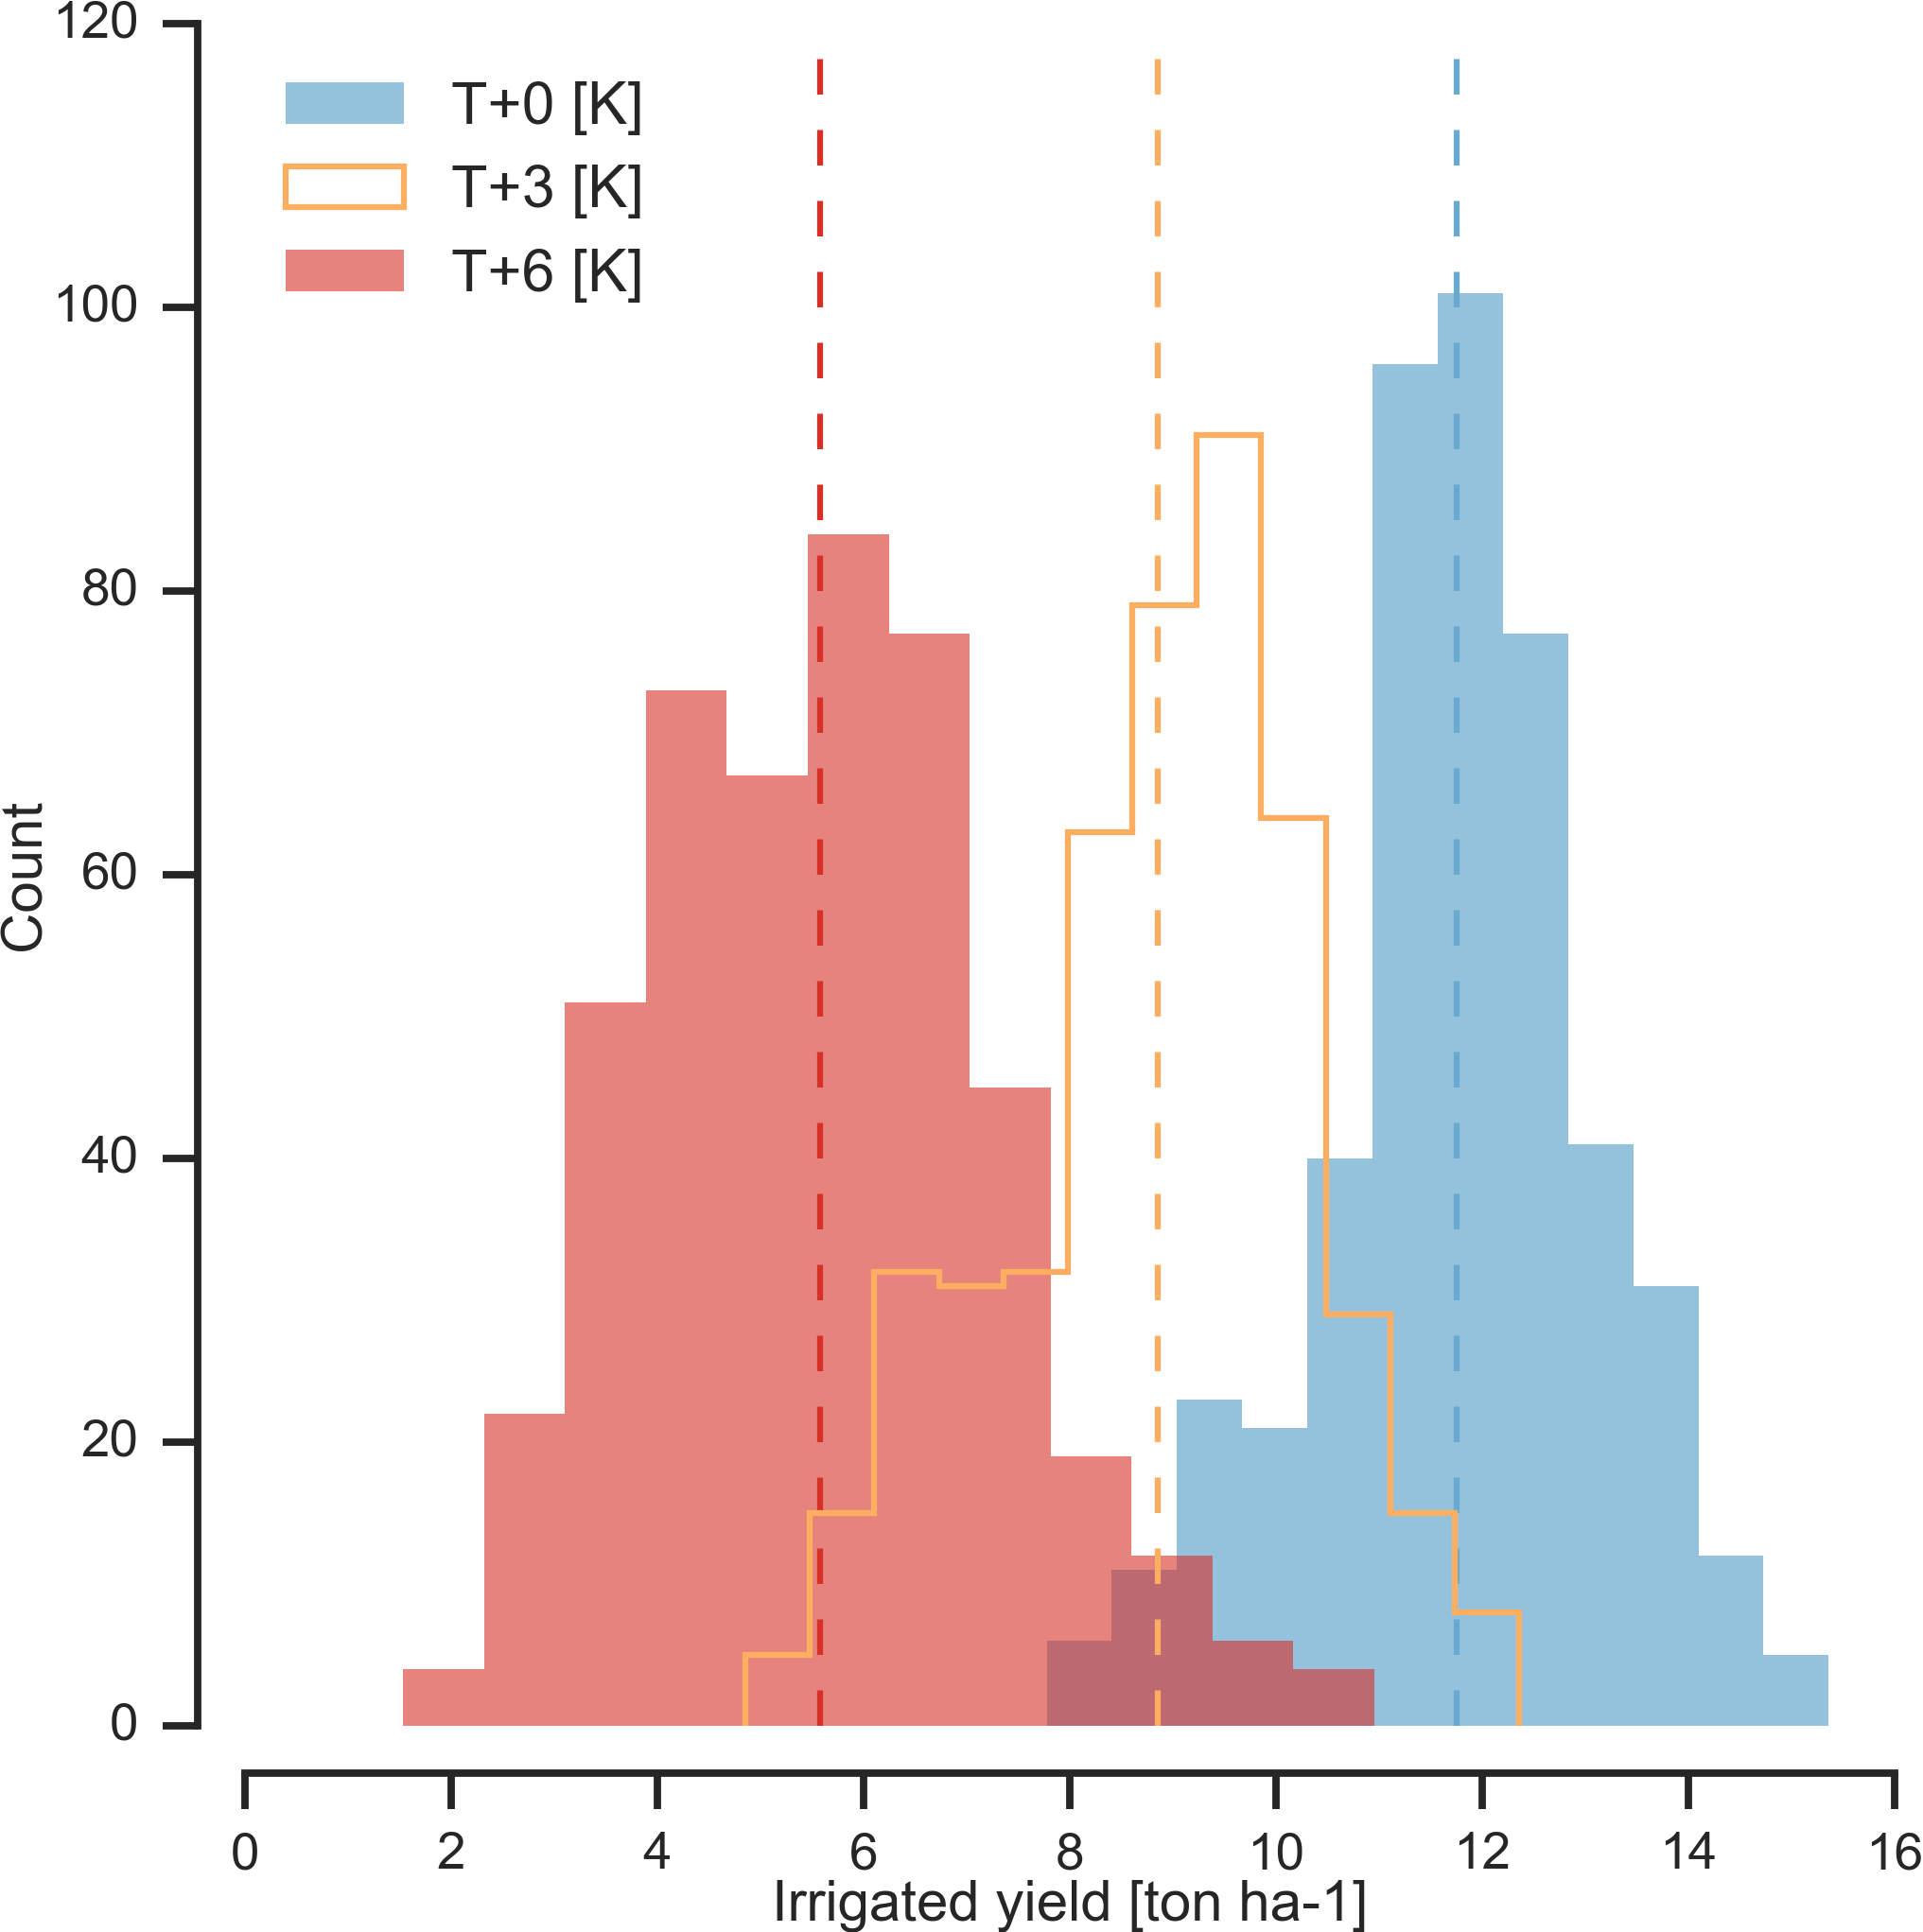
\includegraphics[width=8.3cm]{figures/hist_year.png}
   \caption{
   Example showing results of 
increased crop yield sensitivity to year-over-year climate variations 
under climate stress. Figure shows distributions of yields from examples 
of Figure 1, of irrigated (left) and rainfed (right) maize in Iowa in 
scenarios of altered temperature (left) and precipitation (right)..  
Under large warming (T+6) or drying (P-50\%), increased sensitivity means 
that distributions of year-over-year crop yields widen relative to 
present-day simulations, even though input timeseries has identical 
variance in climate drivers.

   Example showing climatological mean yields and distribution of yearly yields for three 30-year scenarios. 
   Figure shows irrigated maize for nine adjacent high-yield grid cells of Figure \ref{fig:yearvclim} from the pDSSAT model, for the baseline 1981-2010 historical climate (blue) and for scenarios with temperature shifted by T+3 (orange) and T+6 K (red), with other variables held at baseline values. 
   The stronger year-over-year temperature response with higher temperatures seen in Figure \ref{fig:yearvclim} is manifested here as larger variance in annual yields even though the variance in climate drivers is identical. 
   In this work we emulate not the year-over-year distributions but the climatological mean response (dashed vertical lines).
   }
   \label{fig:yearly}
\end{figure}

\begin{figure*}[ht]
\centering
    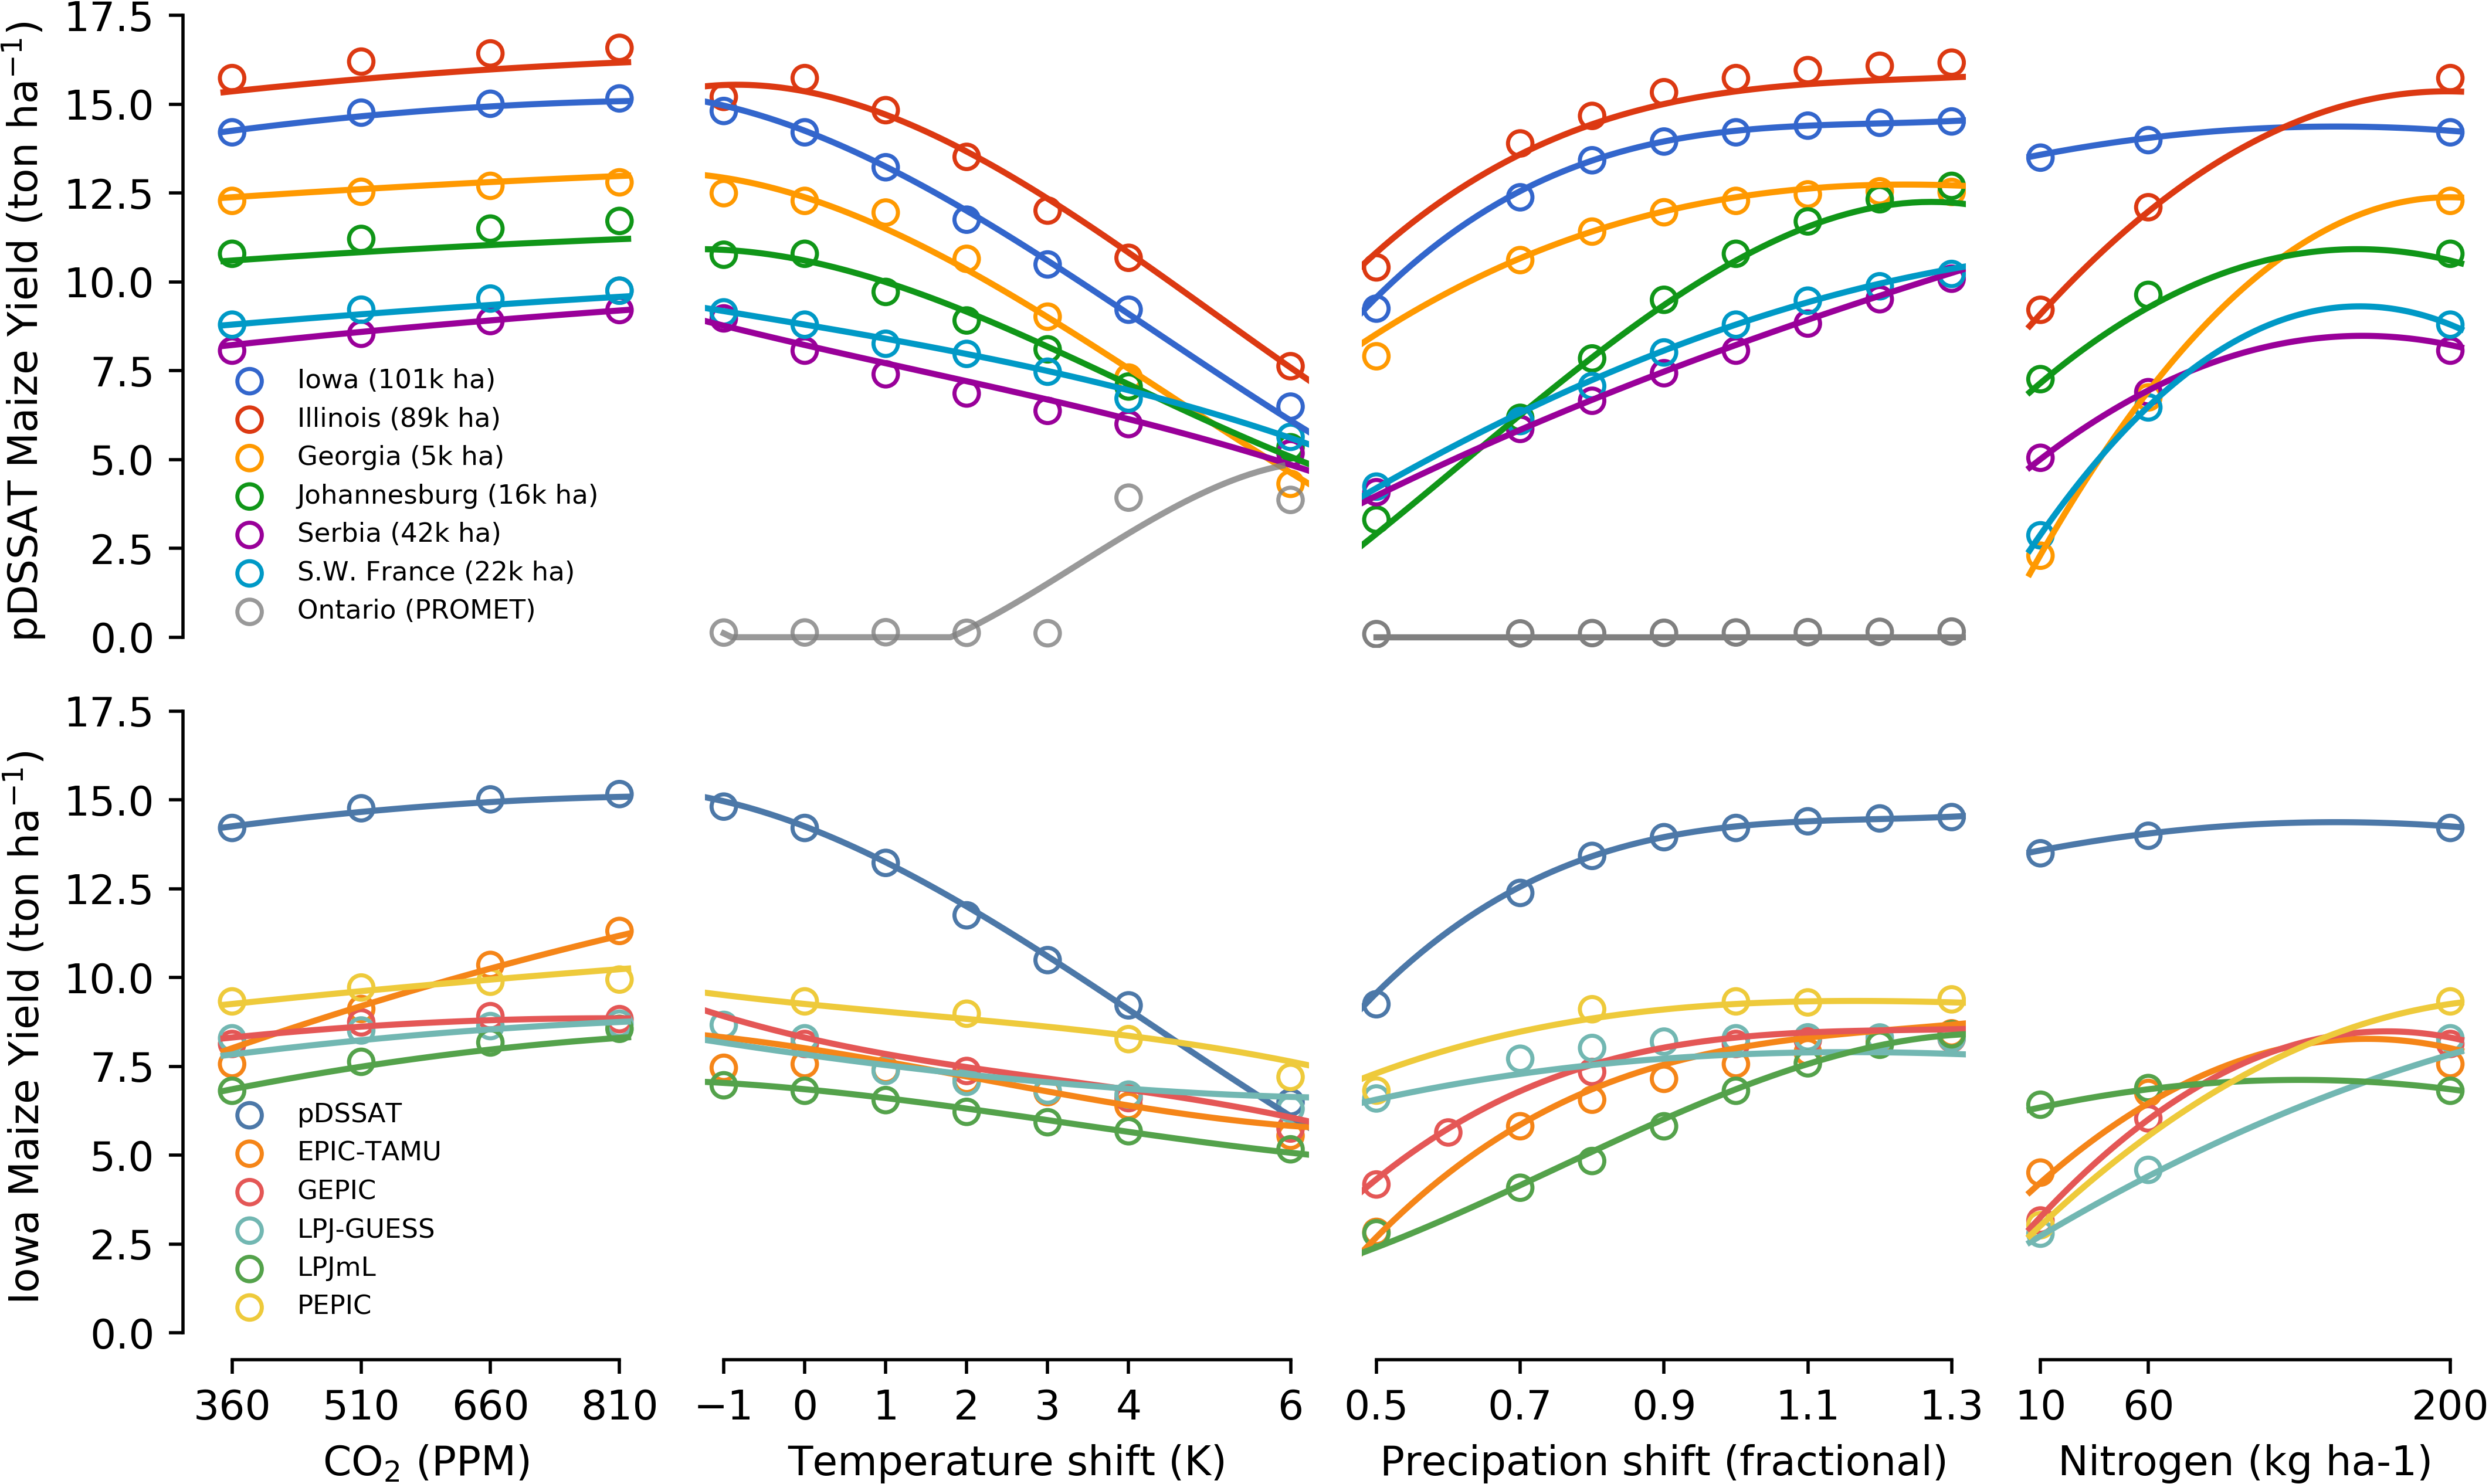
\includegraphics[width=16cm]{figures/regression_example.png}
    \caption{Illustration of spatial and across model variations in yield response successfully captured by the emulator. 
    Top row: simulations and emulations for rainfed maize in the pDSSAT model in six example locations selected to represent high-cultivation areas around the globe. 
    Legend includes hectares cultivated in each selected grid cell. 
    Bottom row: simulations and emulations from six models for rainfed maize in the same Iowa grid cell shown in the top row. 
    Models that do not simulate the nitrogen dimension are omitted for clarity.
    Each panel shows variation along a single variable, with others held at baseline values. 
    Dots show climatological mean yields and lines the results of the full 4D emulator of Equation \ref{eqn:features_original}. 
    In general the climatological response surface is sufficiently smooth that it can be represented within the sampled variable space by the simple polynomial used in this work. 
    While most model responses can readily emulated with a simple polynomial, some response surfaces diverge slightly from the polynomial approach (e.g.\ LPJ-GUESS here) and lead to emulation error, though error generally remains small relative to inter-model uncertainty. 
    The rainfed maize response in north-central Ontario is shown for the PROMET model as a good example of an area where the emulator fails.
    Note that some models are uncalibrated, increasing spread in absolute yields. 
    }
   \label{fig:regression}
\end{figure*}


Finally, we show a damage function constructed from the 4D emulation, aggregated to global yield, with simulated values shown for comparison (Figure \ref{fig:globe_em}, which shows maize on currently cultivated land; see Figures SXX-XX for other crops and dimensions). 
The emulated values closely match simulations even at this aggregation level.


\begin{figure}[ht]
    \centering
    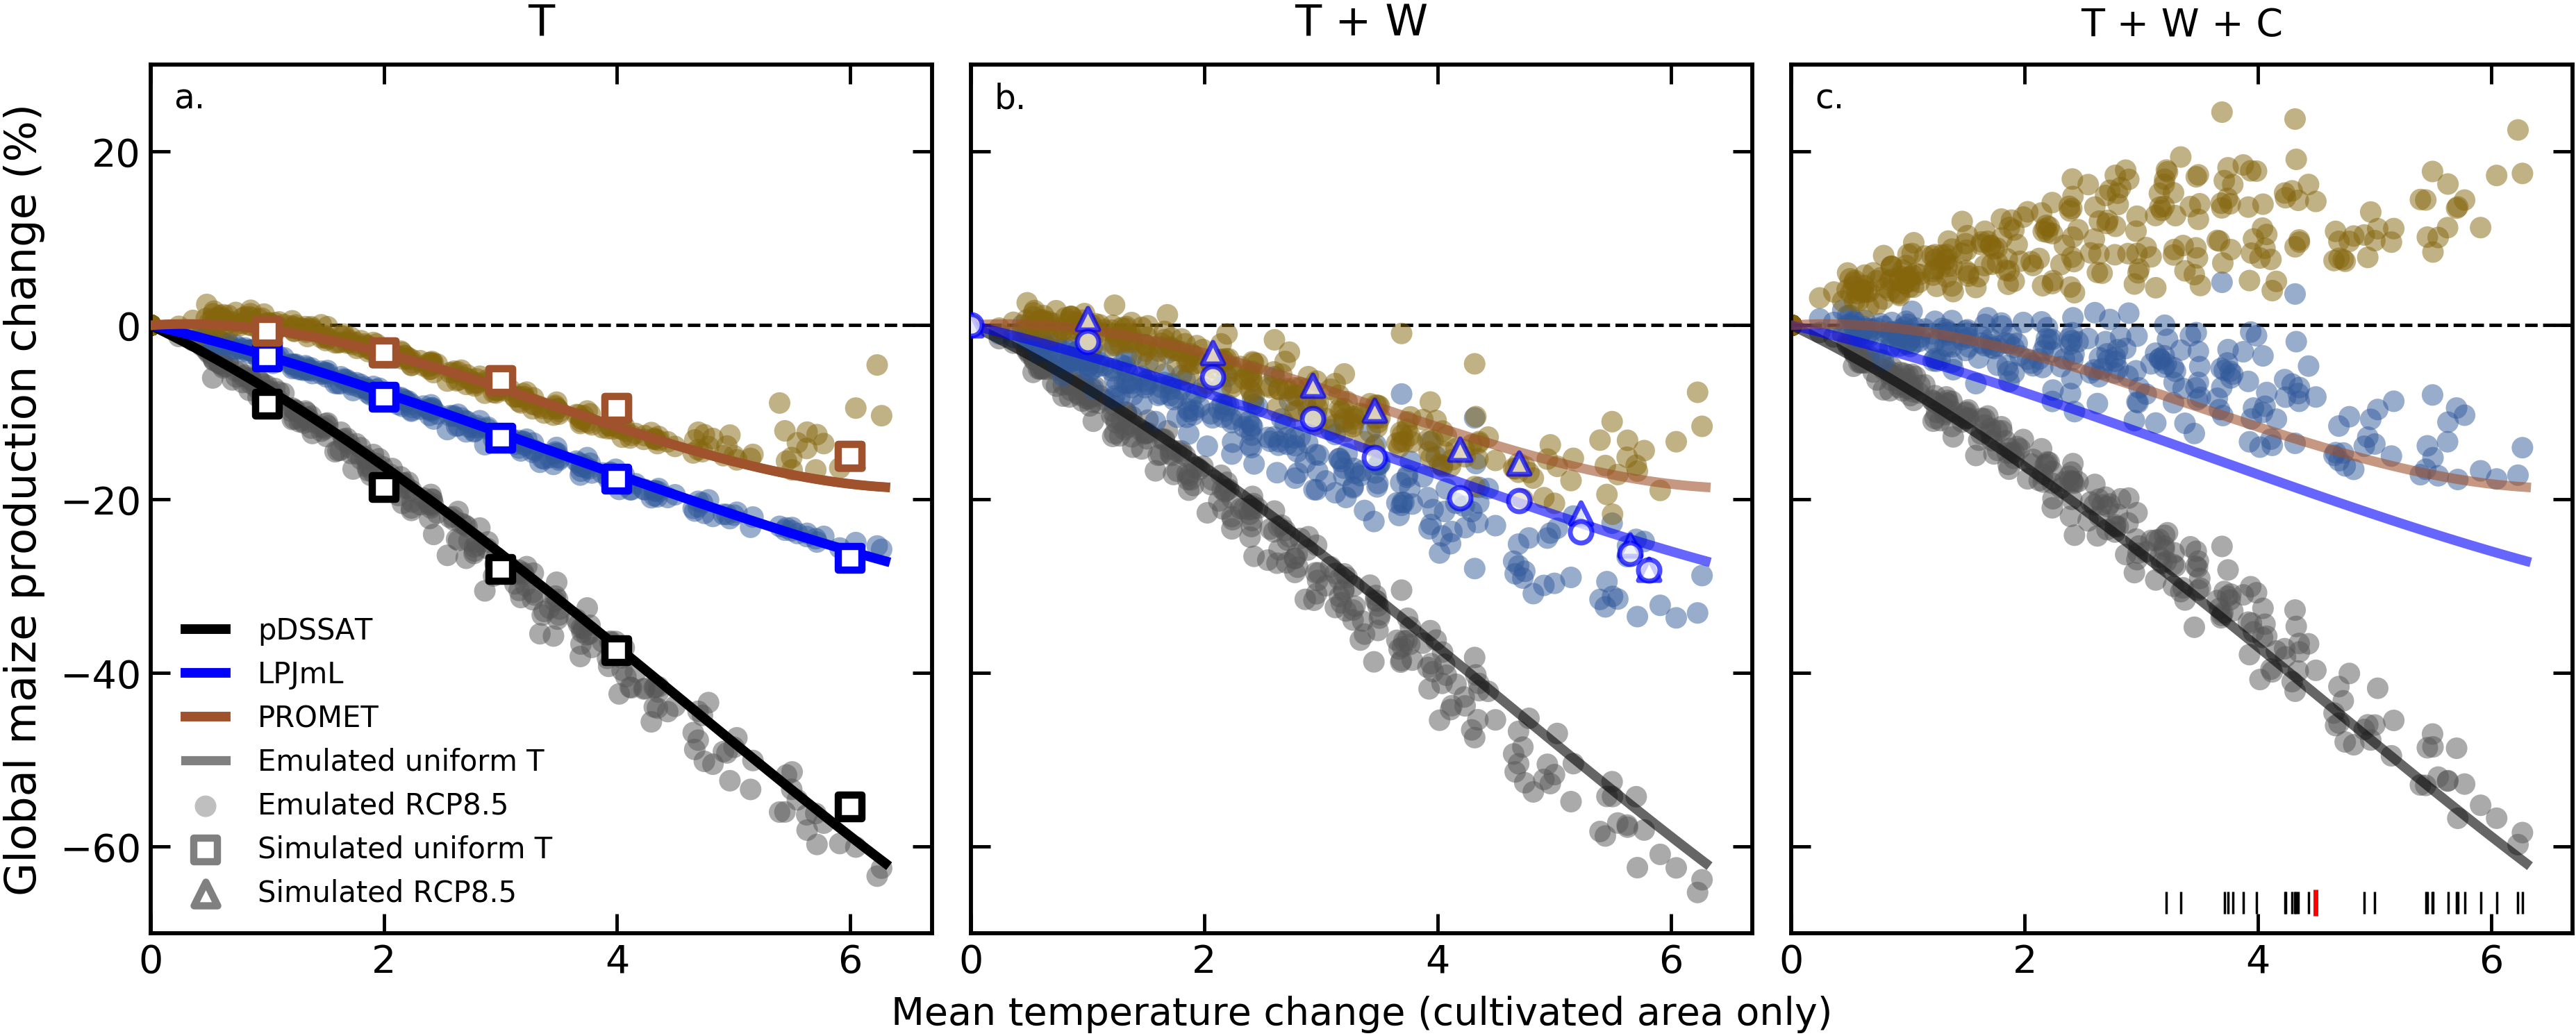
\includegraphics[width=8.3cm]{figures/global_em_maize.png}
    \caption{Global emulated damages for maize on currently cultivated lands for the GGCMI Phase II models emulated, for uniform temperature shifts with other inputs held at baseline. 
    (The damage function is created from aggregating up emulated values at the grid cell level, not from a regression of global mean yields.) 
    Lines are emulations for rainfed (solid) and irrigated (dashed) crops; for comparison, dots are the simulated values for the rainfed case.  
    For most models, irrigated crops show a sharper reduction than rainfed because of the locations of cultivated areas: irrigated crops tend to be grown in warmer areas where impacts are more severe for a given temperature shift (the exceptions are PROMET, JULES, and LPJmL, see \citet{Franke2019a} for more details). 
    For other crops and scenarios see Figures SXX-XX in the supplemental material.}
    \label{fig:globe_em}
\end{figure}

so the section on Figure 1 says, can year-over-year and climatological responses be different? the answer is sometimes yes. For example, in 
Figure 1 the year-over-year responses for temperature are very different from the climatological response. Both are approximately linear over the regime sampled, but different in slope, and and moreover the year-over-year response changes slope as a function of climate state). 
In the precip case, on the other hand, the climatological response is strongly nonlinear, but the year-over-year responses matches it very well. 
These effects are physically reasonable. Crops are very sensitive to daily temperature extrema and year-over-year and climatological changes in mean temperature can be associated with different changes (or lack of changes) in the growing season temperature distribution, and so produce different responses. 
Crops are less sensitive to short-term precipitation changes, since they care about soil moisture and the soil integrates.(cite Glotter et al for showing that in all but very arid regions, crop responses in models are not sensitive to how the precipitation is distributed within a month).


\begin{figure}[ht]
    \centering
    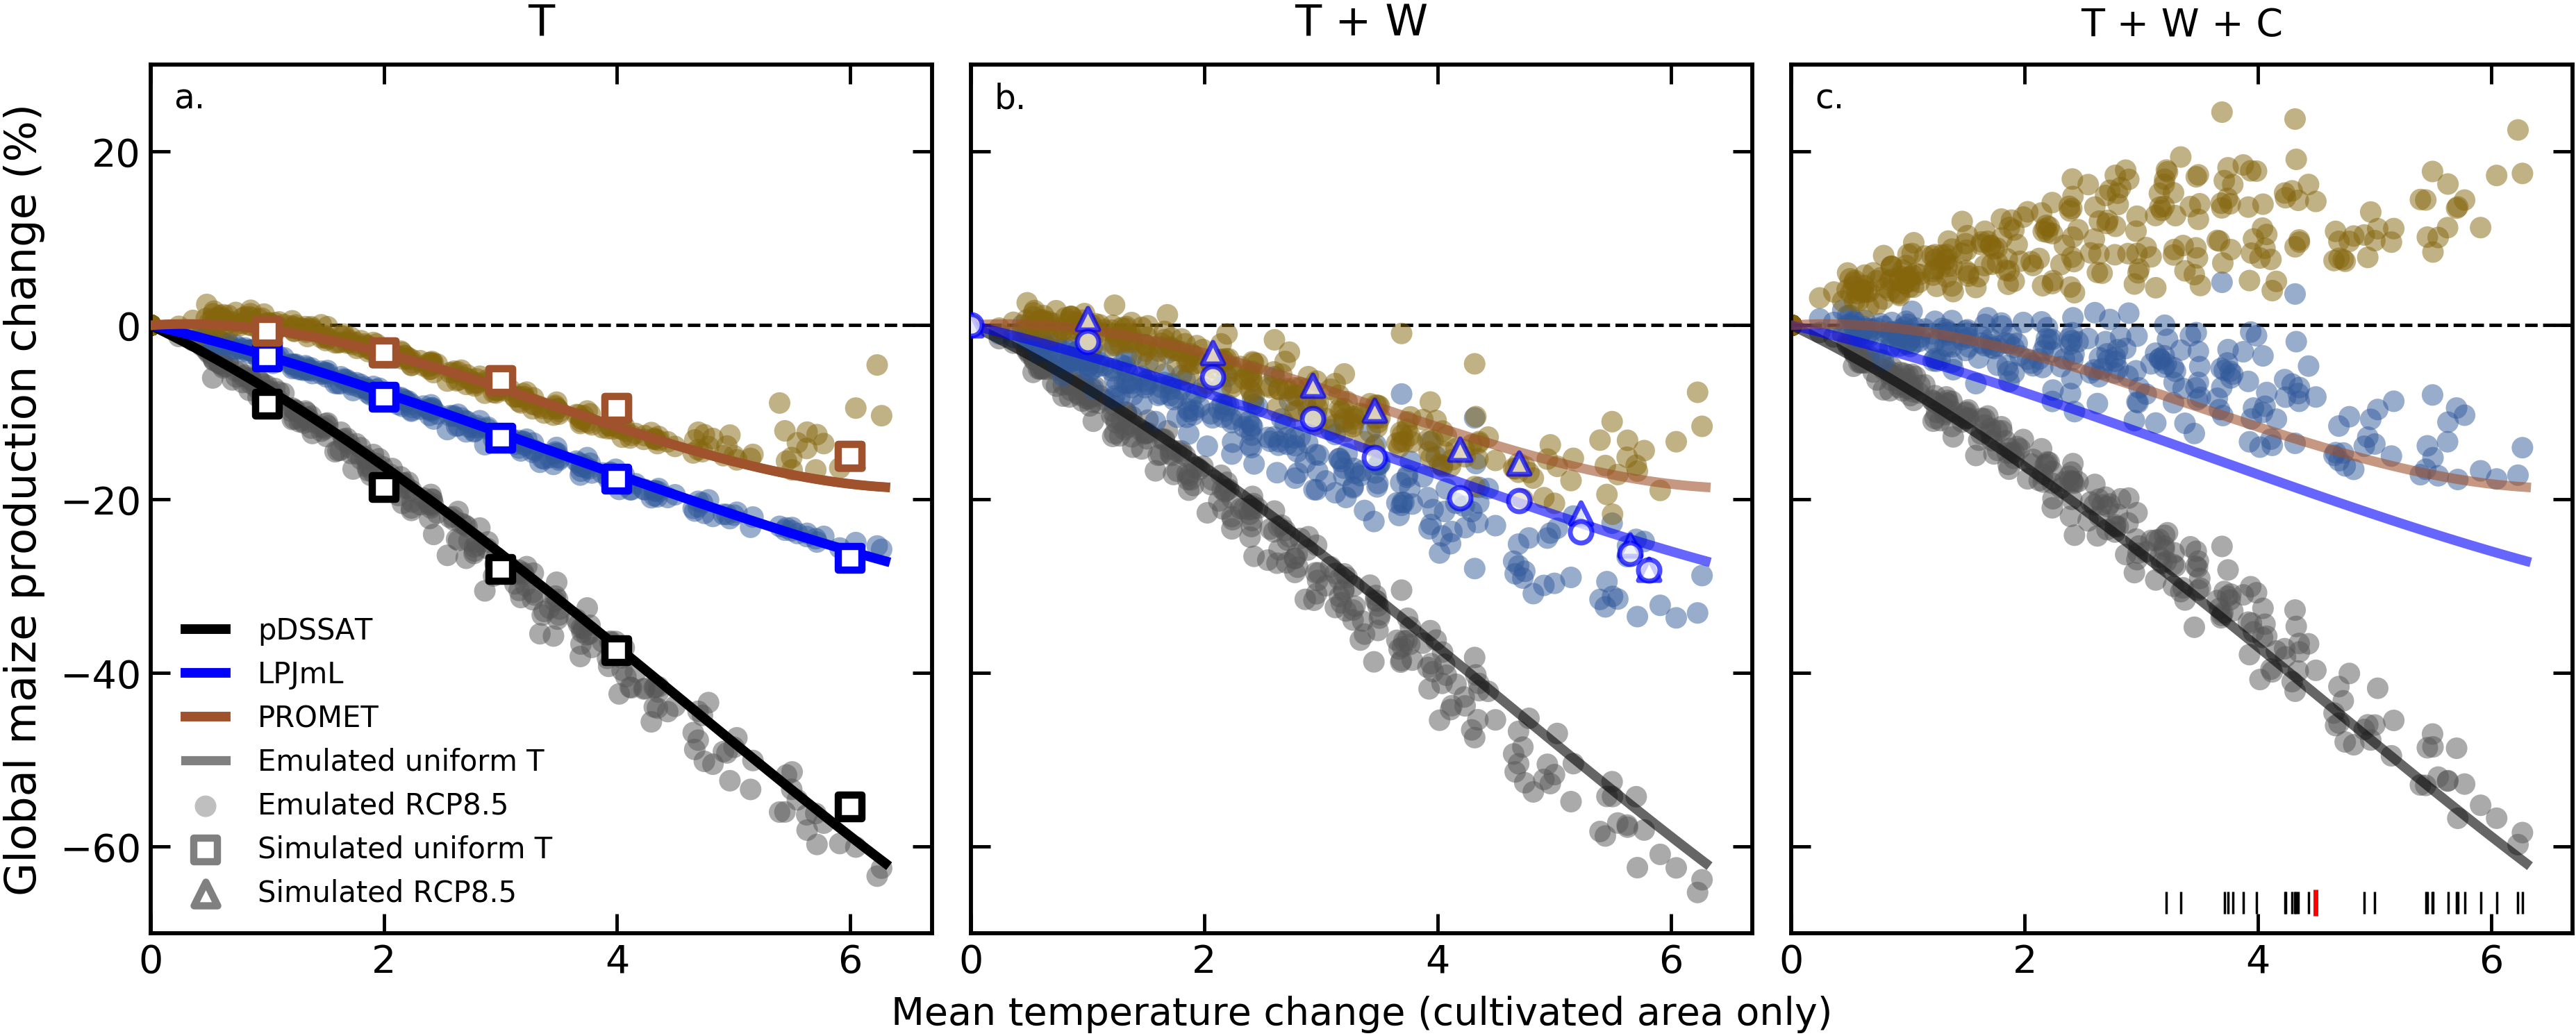
\includegraphics[width = 8.3cm]{figures/global_em_maize.png}
    \caption{Global emulated damages for maize on currently cultivated lands for three example GGCMI Phase II models. 
    Scatter points show the emulated production change from the 1980-2010 mean value for each crop model using inputs from 30 climate models from the CMIP-5 archive \citep{Taylor2012} at the decadal timescale for RCP 8.5.
    The x-axis represents the mean temperature shift over all grid cells where crops are grown (no weighted by cultivation area).
    Temperature and precipitation vary in the climate runs but the effects of CO$_2$ are not included here.
    Open square markers show the Phase II simulated values at each temperature level with other inputs held at baseline values (W+0\%, C = 360ppm, and N = 200kg ha-1).
    Bold lines show emulated values with uniform global temperature shifts applied and precipitation held constant. 
    Rug plots show end of century (2090-2100 mean) values for temperature change for each CMIP-5 model and resultant production change for each crop and climate model combination (including the six models not shown in full).
    In all cases nitrogen is fixed at 200 (kg ha$^-1$) and global production values are aggregated up from the grid cell level based on the growing areas for rainfed and irrigated maize \citep{Portmann2010}. 
    Models not shown: CARAIB, EPIC-TAMU, JULES, GEPIC, LPJ-GUESS, and PEPIC.
    }
    \label{fig

    Global emulated damages for maize on currently cultivated lands for three example GGCMI Phase II models. 
    Scatter points show the emulated production change from the 1980-2010 mean value for each crop model using inputs from 30 climate models from the CMIP-5 archive \citep{Taylor2012} at the decadal timescale for RCP 8.5.
    The x-axis represents the mean temperature shift over all grid cells where crops are grown (no weighted by cultivation area).
    Open square markers show the Phase II simulated values at each temperature level with other inputs held at baseline values (W+0\%, C = 360ppm, and N = 200kg ha-1).
    Bold lines show emulated values with uniform global temperature shifts applied and precipitation and CO$_2$ held constant. 
    Panels a-c show CMIP-5 temperature only, temperature and precipitation, and all three effects respectively. 
    Bold lines are repeated in panels b and c for reference. 
    Rug plots show end of century (2090-2100 mean) values for temperature change for each CMIP-5 model (panel c. only) and the resultant maize production change for each crop and climate model combination (including the additional six crop model emulators not shown in full). 
    Red rug shows the ensemble median value.
    In all cases nitrogen is fixed at 200 (kg ha$^-1$) and global production values are aggregated up from the grid cell level based on the growing areas for rainfed and irrigated maize \citep{Portmann2010}. 

    Illustration of the effects of different factors affecting yields in more realistic climate scenarios. 
    Figures shows emulated damages for maize on currently cultivated lands under RCP8.5 scenarios for three representative crop models, with changes to T only (left), to T and P (center), and to T, P, and CO2 (right)
    Scatter points show the emulated production change from the 1980-2010 mean value for each crop model using inputs from 30 climate models from the CMIP-5 archive \citep{Taylor2012} at the decadal timescale for RCP 8.5.
    The x-axis represents the mean temperature shift over all grid cells where crops are grown (no weighted by cultivation area).
    Open square markers show the Phase II simulated values at each temperature level with other inputs held at baseline values (W+0\%, C = 360ppm, and N = 200kg ha-1).
    Bold lines show emulated values with uniform global temperature shifts applied and precipitation and CO$_2$ held constant. 
    Rug plots show end of century (2090-2100 mean) values for temperature change for each CMIP-5 model (panel c. only) and the resultant maize production change for each crop and climate model combination (including the additional six crop model emulators not shown in full and the red rug is the median). 
    In all cases nitrogen is fixed at 200 (kg ha$^-1$) and global production values are aggregated up from the grid cell level based on the growing areas for rainfed and irrigated maize \citep{Portmann2010}. 
    Models not shown: CARAIB, EPIC-TAMU, JULES, GEPIC, LPJ-GUESS, and PEPIC.
    Emulation is generally successful, except for PROMET at extreme temperature change. Precipitation increases uncertainty across climate model projections and the CO$_2$ response is diverse across crop models.
